% $HeadURL$

%%%%%%%%%%%%%%%%%%%%%%%%%%%%%%%%%%%%%%%%%%%%%%%%%%%%%%%%%%%%%%%%%%%%%%
%%%%                   Complex
%%%%%%%%%%%%%%%%%%%%%%%%%%%%%%%%%%%%%%%%%%%%%%%%%%%%%%%%%%%%%%%%%%%%%%

\subsection{Glyph: \glyph{Complex}}\label{sec:complex}

A \glyph{complex} node represents a biochemical entity composed of other biochemical entities, whether macromolecules, simple chemicals, multimers, or other complexes.  The resulting entity may have its own identity, properties and function in an SBGN diagram.

\begin{glyphDescription}

\glyphSboTerm SBO:0000253 ! non-covalent complex

\glyphContainer A \glyph{complex} possesses its own container box surrounding the juxtaposed container boxes of its components.  This container box is a rectangle with cut-corners (an octagonal box with sides of two different lengths).  The size of the cut-corners are adjusted so that there is no overlap between the container and the components.  The container boxes of the components must not overlap.

\glyphLabel The identification of a \glyph{named complex} is carried by an unbordered box containing a string of characters.  The characters may be distributed on several lines to improve readability, although this is not mandatory.  The label box has to be attached to the midway between the border of the complex's container box and the border of the components' container boxes.

\glyphAux A \glyph{complex} can carry state variables (see \sect{stateVariable}).  The state of a complex is defined by the set of the all its state variable and all the state variables of all its components.  A \glyph{complex} can also carry one or several \glyph{units of information} (see \sect{unitInfo}).  Those units of information can characterize a domain, such as a binding site.  Particular \glyph{units of information} carry the material type and the conceptual type of the macromolecules.  A \glyph{complex} may carry a \glyph{clone marker} (see \sect{cloneMarker}).

\end{glyphDescription}


\begin{figure}[H]
  \centering
  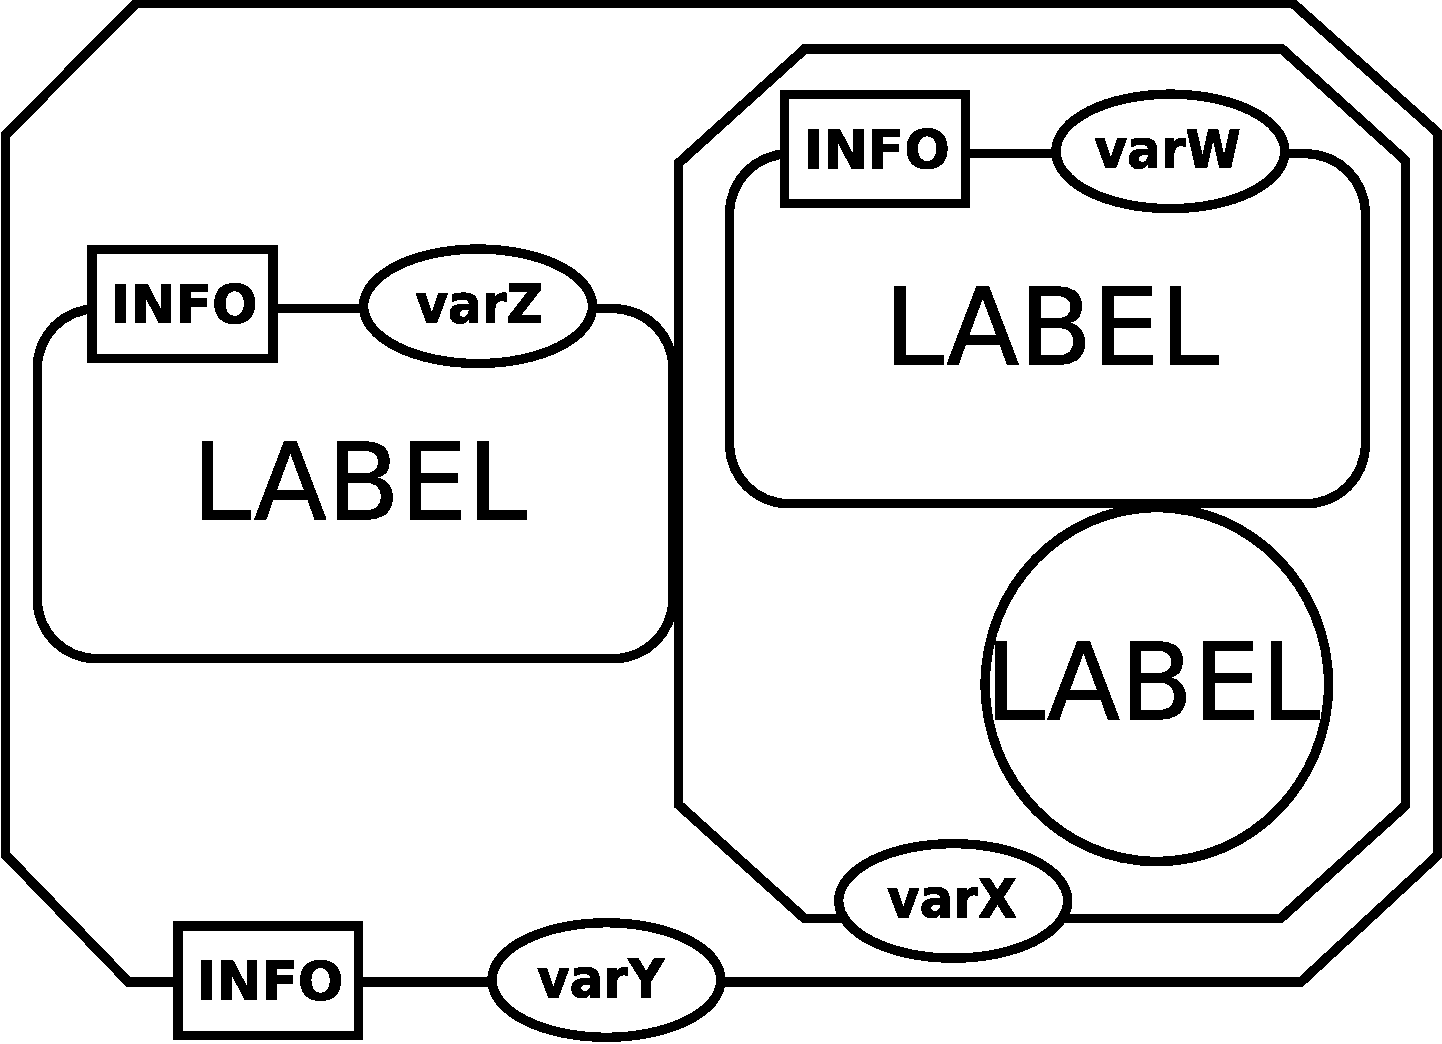
\includegraphics[scale = 0.3]{images/complex}
  \caption{An example \PD glyph for \glyph{complex}.}
  \label{fig:complex}
\end{figure}



% The following is for [X]Emacs users.  Please leave in place.
% Local Variables:
% TeX-master: "../sbgn_PD-level1"
% End:
